\chapter{Conception}
Dans cette partie, nous verrons l’analyse des différences dans l’interface du projet. Ce projet avait pour objectif de développer une application intuitive visant à optimiser l'expérience utilisateur.


\section{ Architecture de la solution JobAI}

L’architecture de JobAI suit une approche modulaire, distribuée et orientée services, articulée autour d’un front-end web React, d’un backend intelligent (LLMs), d’un stockage centralisé dans Firebase, d’une extension Chrome autonome, et d’un agent IA externe pour la postulation automatique. Chaque composant remplit un rôle spécifique et communique avec les autres via des appels API ou des flux de données asynchrones.
Schéma d'interaction entre les composants


\begin{figure}[H]
    \centering
    % \setlength{\fboxrule}{0.5pt} % Épaisseur de la bordure
    % \setlength{\fboxsep}{0pt} % Espace entre image et bordure
    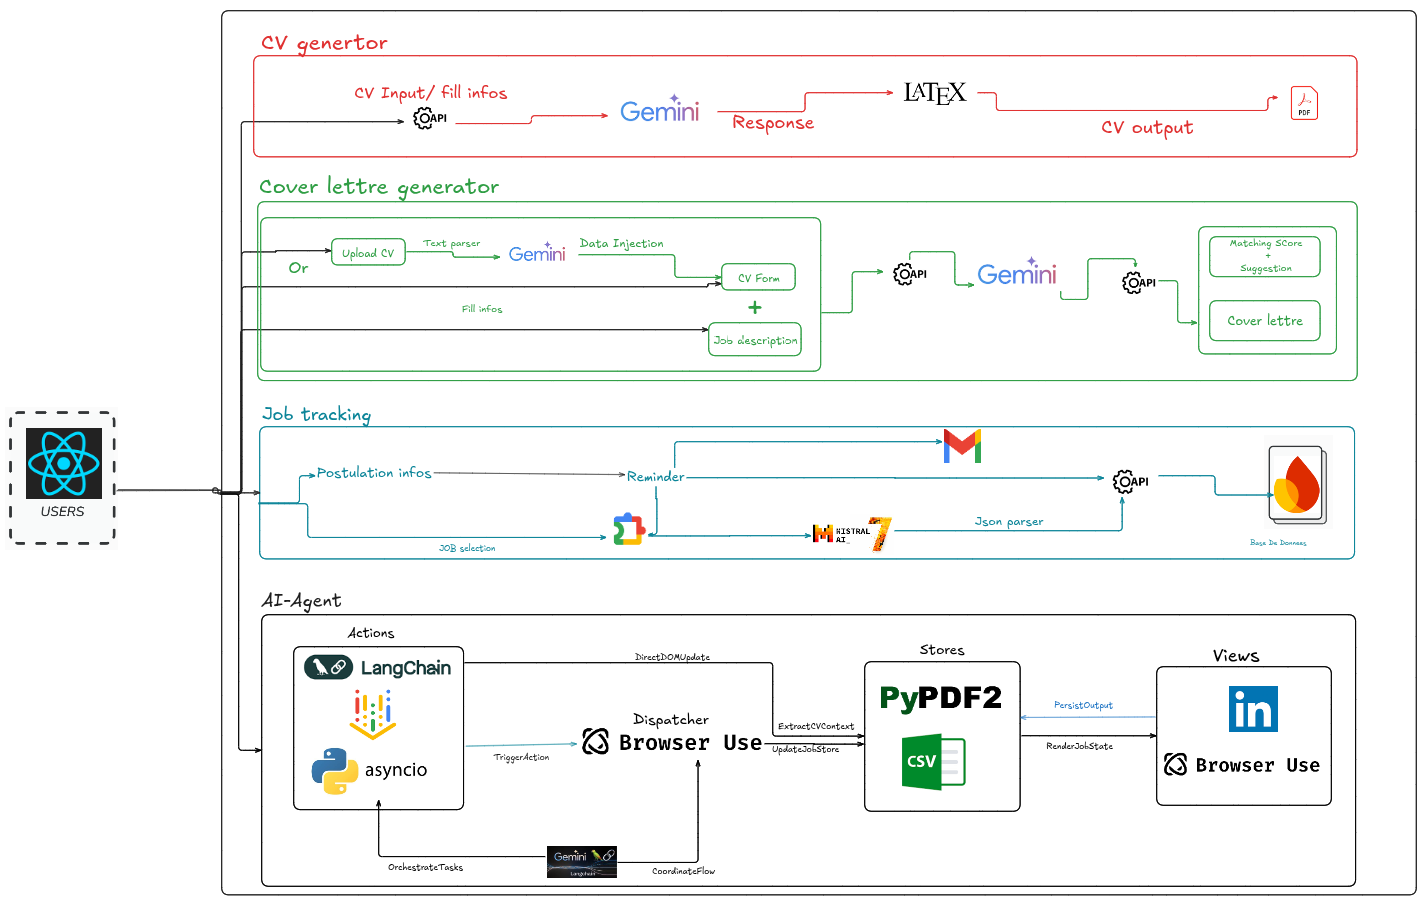
\includegraphics[width=1\linewidth]{screens/archi.png}
    \caption{Architecture de la solution}
    \label{fig: Architecture de la solution}
\end{figure}

\section*{Description détaillée des composants}

\begin{enumerate}
    \item \textbf{Interface Utilisateur Web – React.js + Tailwind CSS} \\
    Point d'entrée de l'utilisateur sur la plateforme JobAI permettant :\\
L'interface utilisateur web constitue le point d'entrée principal de l'utilisateur sur la plateforme JobAI. Développée avec React.js et stylisée avec Tailwind CSS, elle permet aux utilisateurs de renseigner manuellement leurs informations personnelles, expériences, compétences et préférences. Les utilisateurs peuvent également générer des CV ou lettres de motivation à partir des données saisies ou d'un CV importé. L'interface offre un tableau de bord intuitif pour consulter et suivre les candidatures, configurer les préférences de l'agent IA autonome, et interagir avec les modèles LLM à travers un design soigné et accessible.

    \item \textbf{Modèles de langage (LLMs)} \\
    Utilisés dans plusieurs processus clés :
Les modèles de langage sont utilisés dans plusieurs processus clés de la plateforme. Ils permettent la génération de CV à partir des informations fournies par l'utilisateur et la rédaction de lettres de motivation personnalisées selon l'offre d'emploi ciblée. Ces modèles réalisent également l'analyse sémantique permettant d'évaluer la compatibilité entre le profil du candidat et l'offre d'emploi, produisant un score de matching pertinent. Ils assurent aussi le parsing sémantique des descriptions d'offres capturées depuis l'extension, les structurant en format JSON exploitable. Ces modèles sont appelés via des fonctions backend ou microservices avec des prompts spécifiquement adaptés à chaque tâche.


    \item \textbf{Base de données cloud \& Authentification – Firebase} \\
    La base de données cloud Firebase constitue la brique centrale du stockage de l'application. Elle assure une authentification sécurisée via email/password ou OAuth et utilise Firestore pour stocker les données essentielles : profils utilisateurs, CV générés, lettres de motivation, offres sauvegardées et candidatures en cours. Cette infrastructure permet une gestion en temps réel des mises à jour concernant les offres, candidatures et logs de l'agent IA. Firebase offre une scalabilité naturelle et s'intègre de façon fluide avec React, simplifiant considérablement l'architecture technique de la solution.\\

    \item \textbf{Extension Chrome (JavaScript – Manifest V3)} \\
L'extension Chrome fonctionne comme un assistant embarqué directement dans le navigateur pour faciliter la collecte d'offres d'emploi. Elle propose une interface contextuelle qui s'active lors de la sélection d'offres sur des plateformes comme LinkedIn ou Indeed. L'extension extrait automatiquement les informations clés telles que le poste, l'entreprise et la localisation, puis envoie ces données à un backend LLM pour structuration en format JSON. Les offres sont ensuite sauvegardées dans Firebase sous l'espace personnel de l'utilisateur, permettant ainsi une centralisation rapide des opportunités professionnelles sans effort manuel significatif.\\


    \item \textbf{Agent IA autonome – Python + useBrowser} \\
L'agent IA autonome représente l'élément le plus innovant de la plateforme. Développé avec Python et la technologie useBrowser, il permet une navigation automatique sur des plateformes comme LinkedIn via un navigateur headless. Cet agent récupère les offres correspondant aux préférences définies par l'utilisateur, génère des candidatures complètes incluant CV et lettre de motivation adaptés, et peut même remplir automatiquement les formulaires pour postuler. Toutes les tentatives de postulation, qu'elles soient réussies ou non, sont journalisées dans Firebase pour assurer un suivi transparent. Son fonctionnement repose sur useBrowser qui combine efficacement l'automatisation du navigateur et les capacités des LLM.\\

    \item \textbf{Avantages de cette architecture}\\
Cette architecture présente de nombreux avantages stratégiques. Sa modularité permet une évolution ou un remplacement indépendant des composants, comme une éventuelle migration de Firebase vers MongoDB si nécessaire. La scalabilité est assurée par un backend cloud et des fonctions IA capables de monter en charge facilement selon les besoins. L'expérience utilisateur reste fluide grâce à la combinaison judicieuse d'automatisation, d'intelligence artificielle et de simplicité d'utilisation. Enfin, l'extensibilité de la plateforme permet d'envisager l'ajout d'autres agents pour des plateformes supplémentaires comme Indeed ou Welcome to the Jungle, élargissant ainsi progressivement sa couverture du marché de l'emploi.\\

\end{enumerate}

\section{Cas d'utilisation – Vue globale}
% \vspace{-1cm}
\begin{figure}[H]
    \centering
    \setlength{\fboxrule}{1pt} % Épaisseur de la bordure
    \setlength{\fboxsep}{0pt} % Espace entre image et bordure
    \fbox{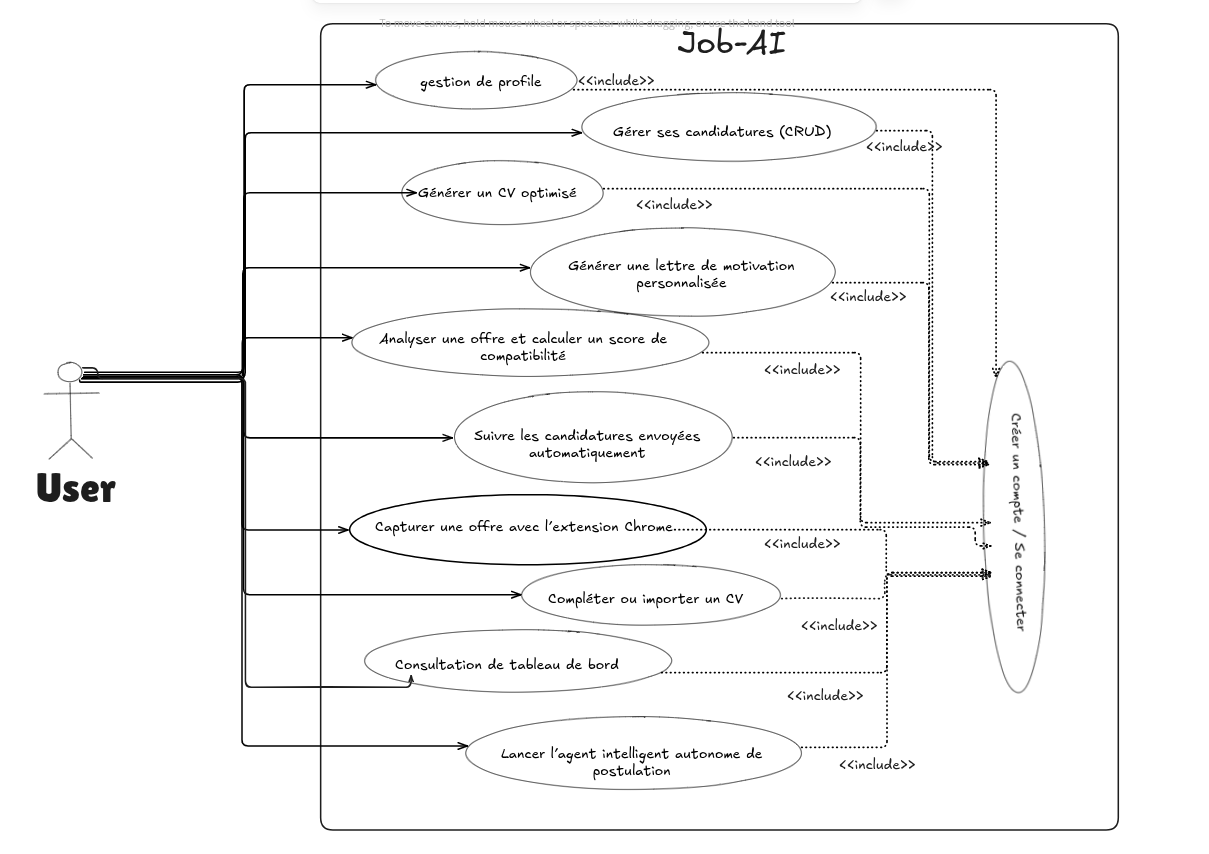
\includegraphics[width=0.8\linewidth]{screens/UseCase.png}}
    \caption{Diagramme des cas d'utilisation de JobAI}
    \label{fig:use_case}
\end{figure}


\begin{enumerate}
    \item \textbf{Créer un compte / Se connecter}
    \begin{itemize}
        \item \textbf{Objectif} : Accéder aux fonctionnalités personnalisées
        \item \textbf{Flux} :
        \begin{itemize}
            \item Inscription via email/mot de passe (Firebase Auth) ou SSO (Google/GitHub)
            \item Validation de l'email
        \end{itemize}
    \end{itemize}

    \item \textbf{Compléter ou importer un CV}
    \begin{itemize}
        \item \textbf{Flux} :
        \begin{itemize}
            \item Import : Téléversement d'un PDF $\rightarrow$ extraction automatique des données
            \item Édition manuelle : Ajout/suppression d'expériences, compétences, formations
        \end{itemize}
    \end{itemize}

    \item \textbf{Générer un CV optimisé}
    \begin{itemize}
        \item \textbf{Déclencheur} : Besoin d'adapter son CV à une offre spécifique
        \item \textbf{Flux} :
        \begin{itemize}
            \item Sélection d'un modèle
            \item Analyse des mots-clés de l'offre $\rightarrow$ suggestions d'optimisation (score ATS)
            \item Génération en PDF avec prévisualisation
        \end{itemize}
    \end{itemize}

    \item \textbf{Analyser une offre et calculer un score de compatibilité}
    \begin{itemize}
        \item \textbf{Flux} :
        \begin{itemize}
            \item Extraction des compétences/requis $\rightarrow$ comparaison avec le profil utilisateur
            \item Affichage d'un score \% (ex: "90\%")
            \item Suggestions pour améliorer la compatibilité
        \end{itemize}
    \end{itemize}

    \item \textbf{Gérer ses candidatures (CRUD)}
    \begin{itemize}
        \item \textbf{Objectif} : Suivre l'état des postulations
        \item \textbf{Flux} :
        \begin{itemize}
            \item Ajout : Manuel (formulaire) ou automatique (via extension/agent)
            \item Mise à jour : Changement de statut (ex: "Entretien prévu le 12/05")
            \item Rappel : Notifications email (Gmail API) selon dates configurées
            \item Suppression : Archivage ou suppression définitive
        \end{itemize}
    \end{itemize}

    \item \textbf{Capturer une offre avec l'extension Chrome}
    \begin{itemize}
        \item \textbf{Déclencheur} : Navigation sur un site d'emploi (Indeed, LinkedIn...)
        \item \textbf{Flux} :
        \begin{itemize}
            \item Clique sur l'extension $\rightarrow$ capture du titre, entreprise, description
            \item Pré-remplissage dans la plateforme $\rightarrow$ validation/édition par l'utilisateur
        \end{itemize}
    \end{itemize}

    \item \textbf{Lancer l'agent intelligent autonome de postulation}
    \begin{itemize}
        \item \textbf{Déclencheur} : Activation de l'automatisation pour une offre
        \item \textbf{Flux} :
        \begin{itemize}
            \item Paramétrage : CV/lettre par défaut, filtres (salaire, localisation)
        \end{itemize}
    \end{itemize}

    \item \textbf{Suivre les candidatures envoyées automatiquement}
    \begin{itemize}
        \item Auditer les candidatures automatiques et éviter les doublons
    \end{itemize}
\end{enumerate}

\textbf{Interconnexion des fonctionnalités} : \\
Les fonctionnalités sont accessibles depuis l'interface principale et interconnectées (ex: la génération de lettre nécessite un CV et/ou une offre).


\section{Diagramme de séquence – Génération de CV}

\begin{figure}[H]
    \centering
    \setlength{\fboxrule}{1pt} % Épaisseur de la bordure
    \setlength{\fboxsep}{0pt} % Espace entre image et bordure
    \fbox{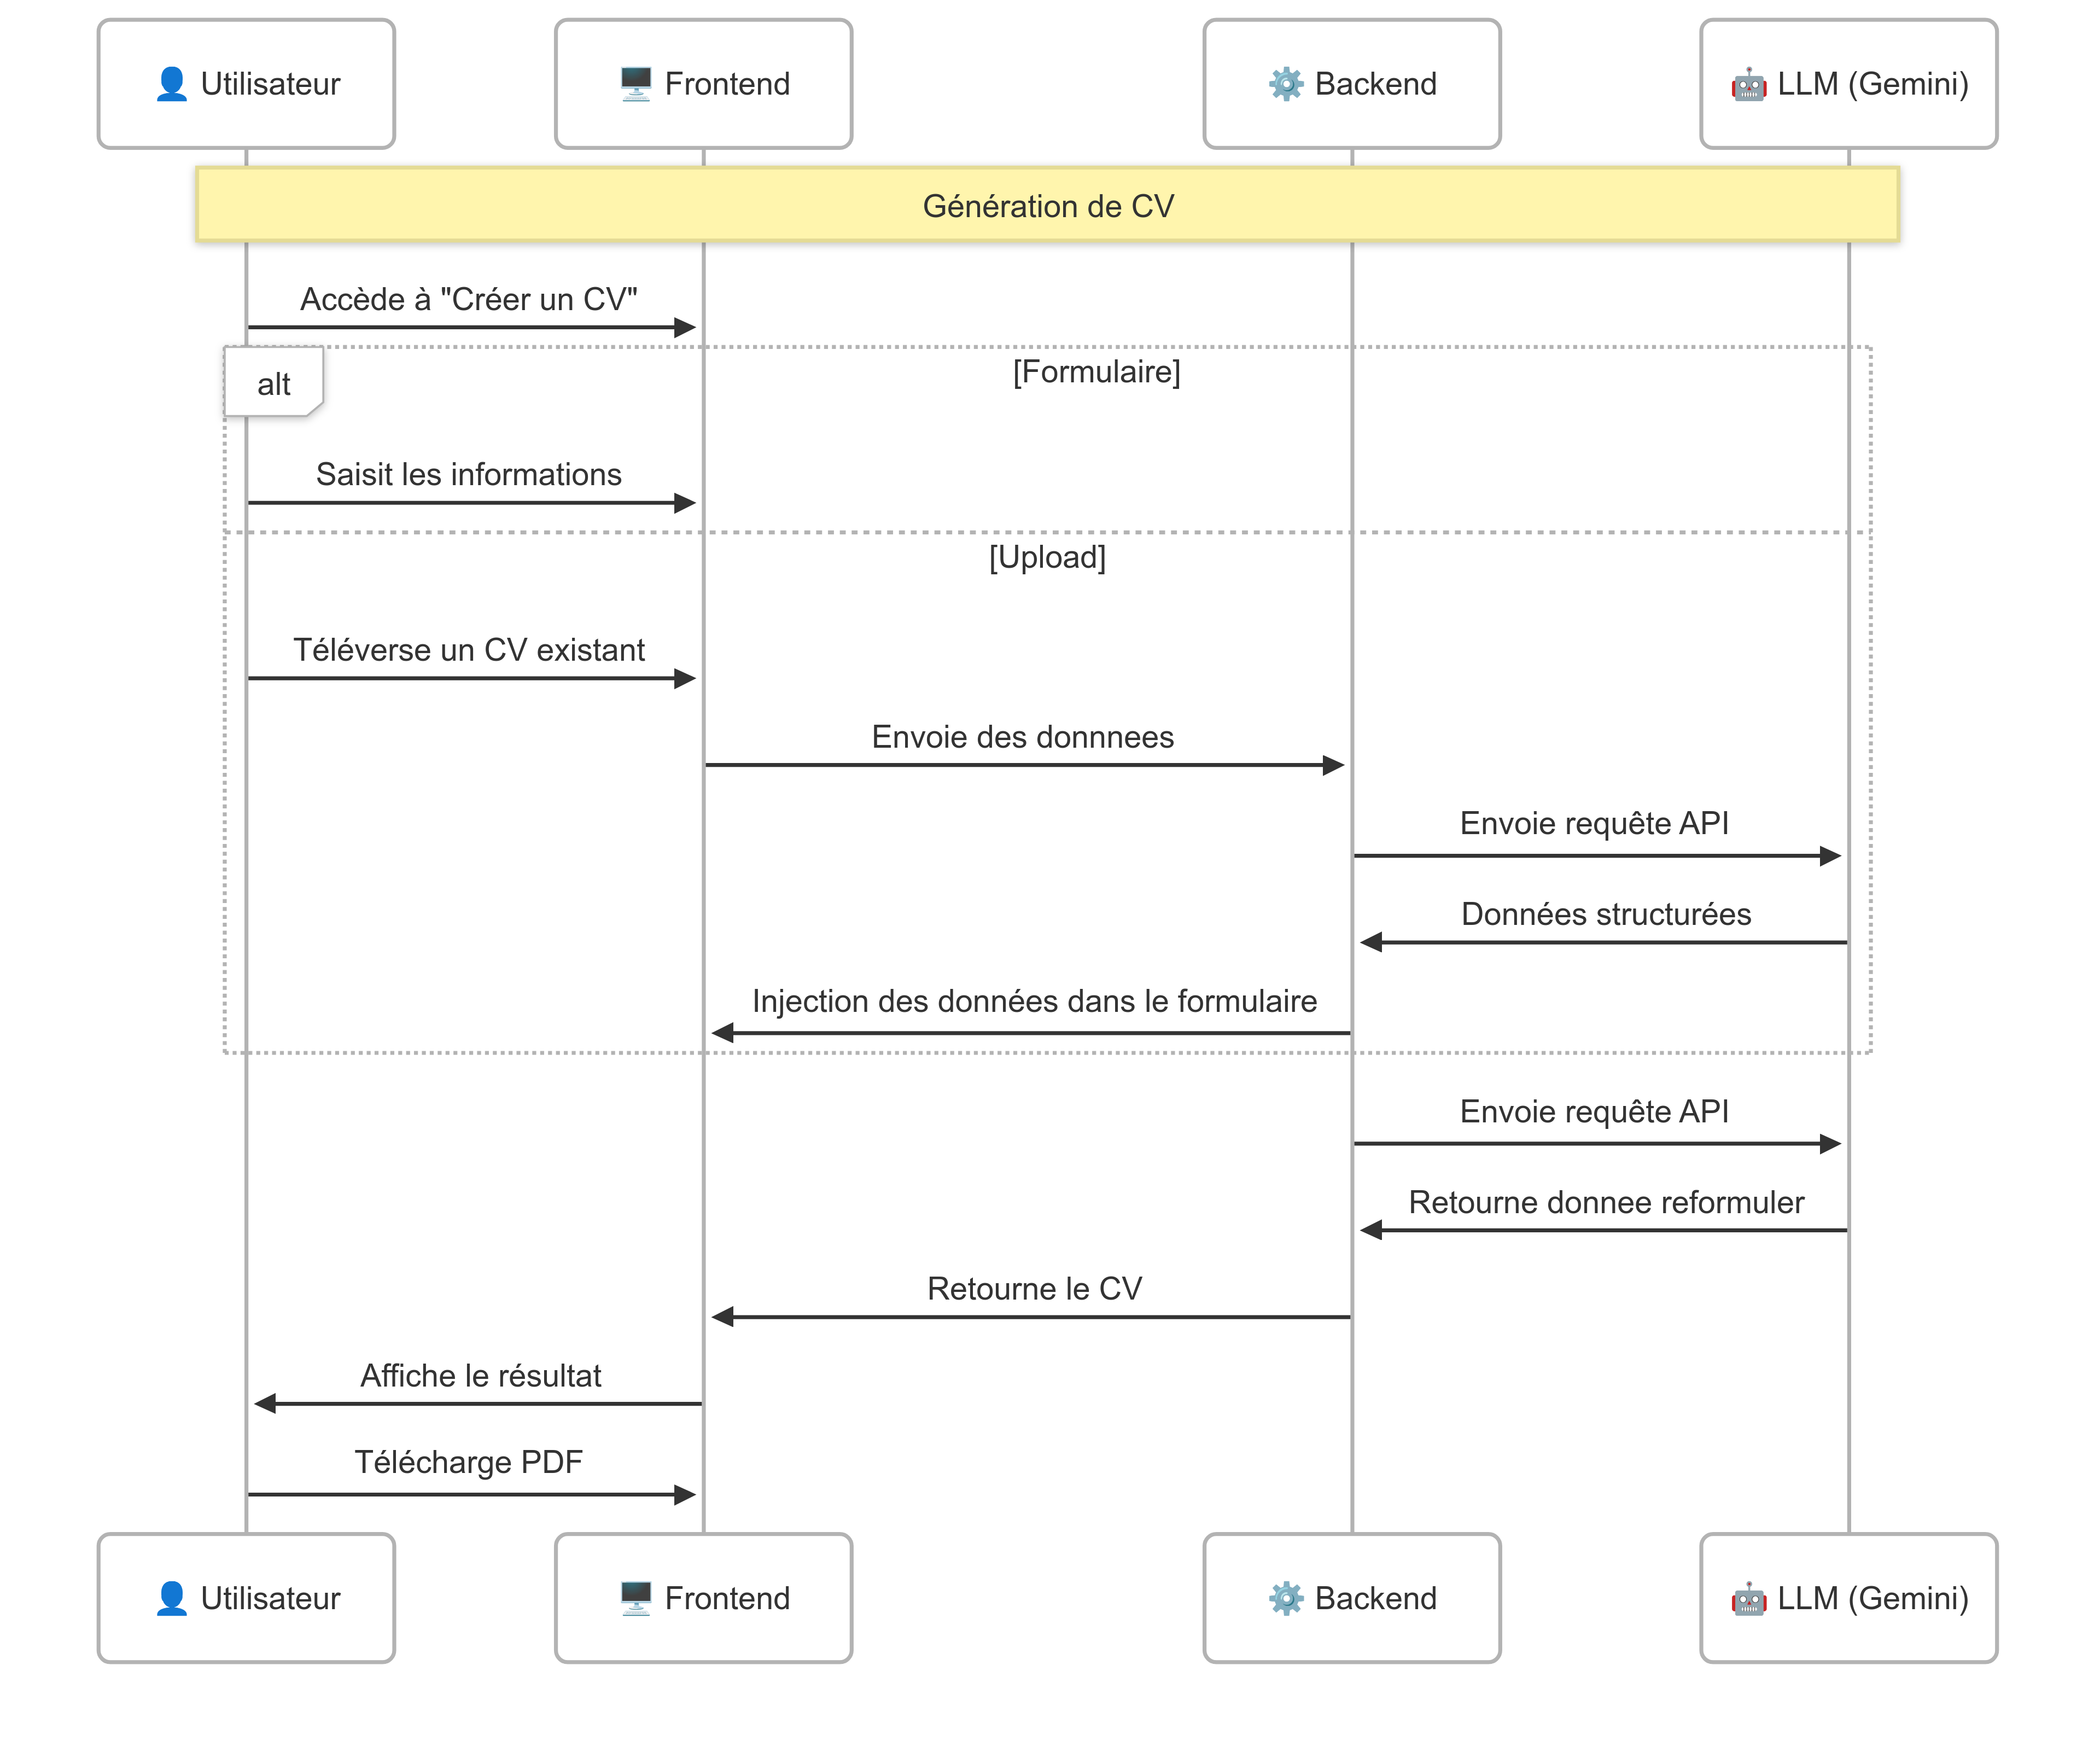
\includegraphics[width=1\linewidth]{screens/sequence-CV.png}}
    \caption{Architecture de la solution}
    \label{fig:Architecture_de_la_solution}
\end{figure}

\subsection*{Acteurs}
\begin{itemize}
    \item Utilisateur
    \item Interface Frontend
    \item Service Backend
    \item Modèle LLM (API IA)
\end{itemize}

\subsection*{Étapes du scénario}
\begin{enumerate}
    \item L'utilisateur accède à la fonctionnalité \og Créer un CV \fg{} depuis le tableau de bord
    
    \item Il choisit entre :
    \begin{itemize}
        \item Remplir un formulaire manuellement

                \item Téléverser un CV existant
    \end{itemize}
    \item Le Frontend transmet les données saisies ou le fichier au Backend
    
    \item Le Backend transforme les données en prompt structuré pour l'API IA
    
    \item Appel au modèle LLM via requête API (Gemini)
    
    \item Le modèle IA retourne un CV formaté selon les bonnes pratiques
    
    \item Le résultat est retourné au Frontend pour visualisation
    
    \item L'utilisateur peut :
    \begin{itemize}
        \item Télécharger le CV généré
        \item L'utiliser directement pour postuler
    \end{itemize}
\end{enumerate}

\subsection*{Flux alternatif}
\begin{itemize}
    \item \textbf{Échec de génération} : Si le modèle LLM ne retourne pas de résultat valide :
    \begin{enumerate}
        \item Le Backend envoie une notification d'erreur au Frontend
        \item L'interface propose à l'utilisateur de réessayer ou de modifier ses données
    \end{enumerate}
    
    \item \textbf{Optimisation supplémentaire} : L'utilisateur peut demander :
    \begin{itemize}
        \item Une version plus concise
        \item Une adaptation à un secteur spécifique
        \item Une traduction dans une autre langue
    \end{itemize}
\end{itemize}
\clearpage
\section{Diagramme de séquence – Cover Lettre}
Ce cas d'usage détaille le processus de génération automatisée d'une lettre de motivation personnalisée en exploitant les informations du CV utilisateur et les détails d'une offre d'emploi spécifique.
\begin{figure}[H]
    \centering
    \setlength{\fboxrule}{1pt} % Épaisseur de la bordure
    \setlength{\fboxsep}{0pt} % Espace entre image et bordure
    \fbox{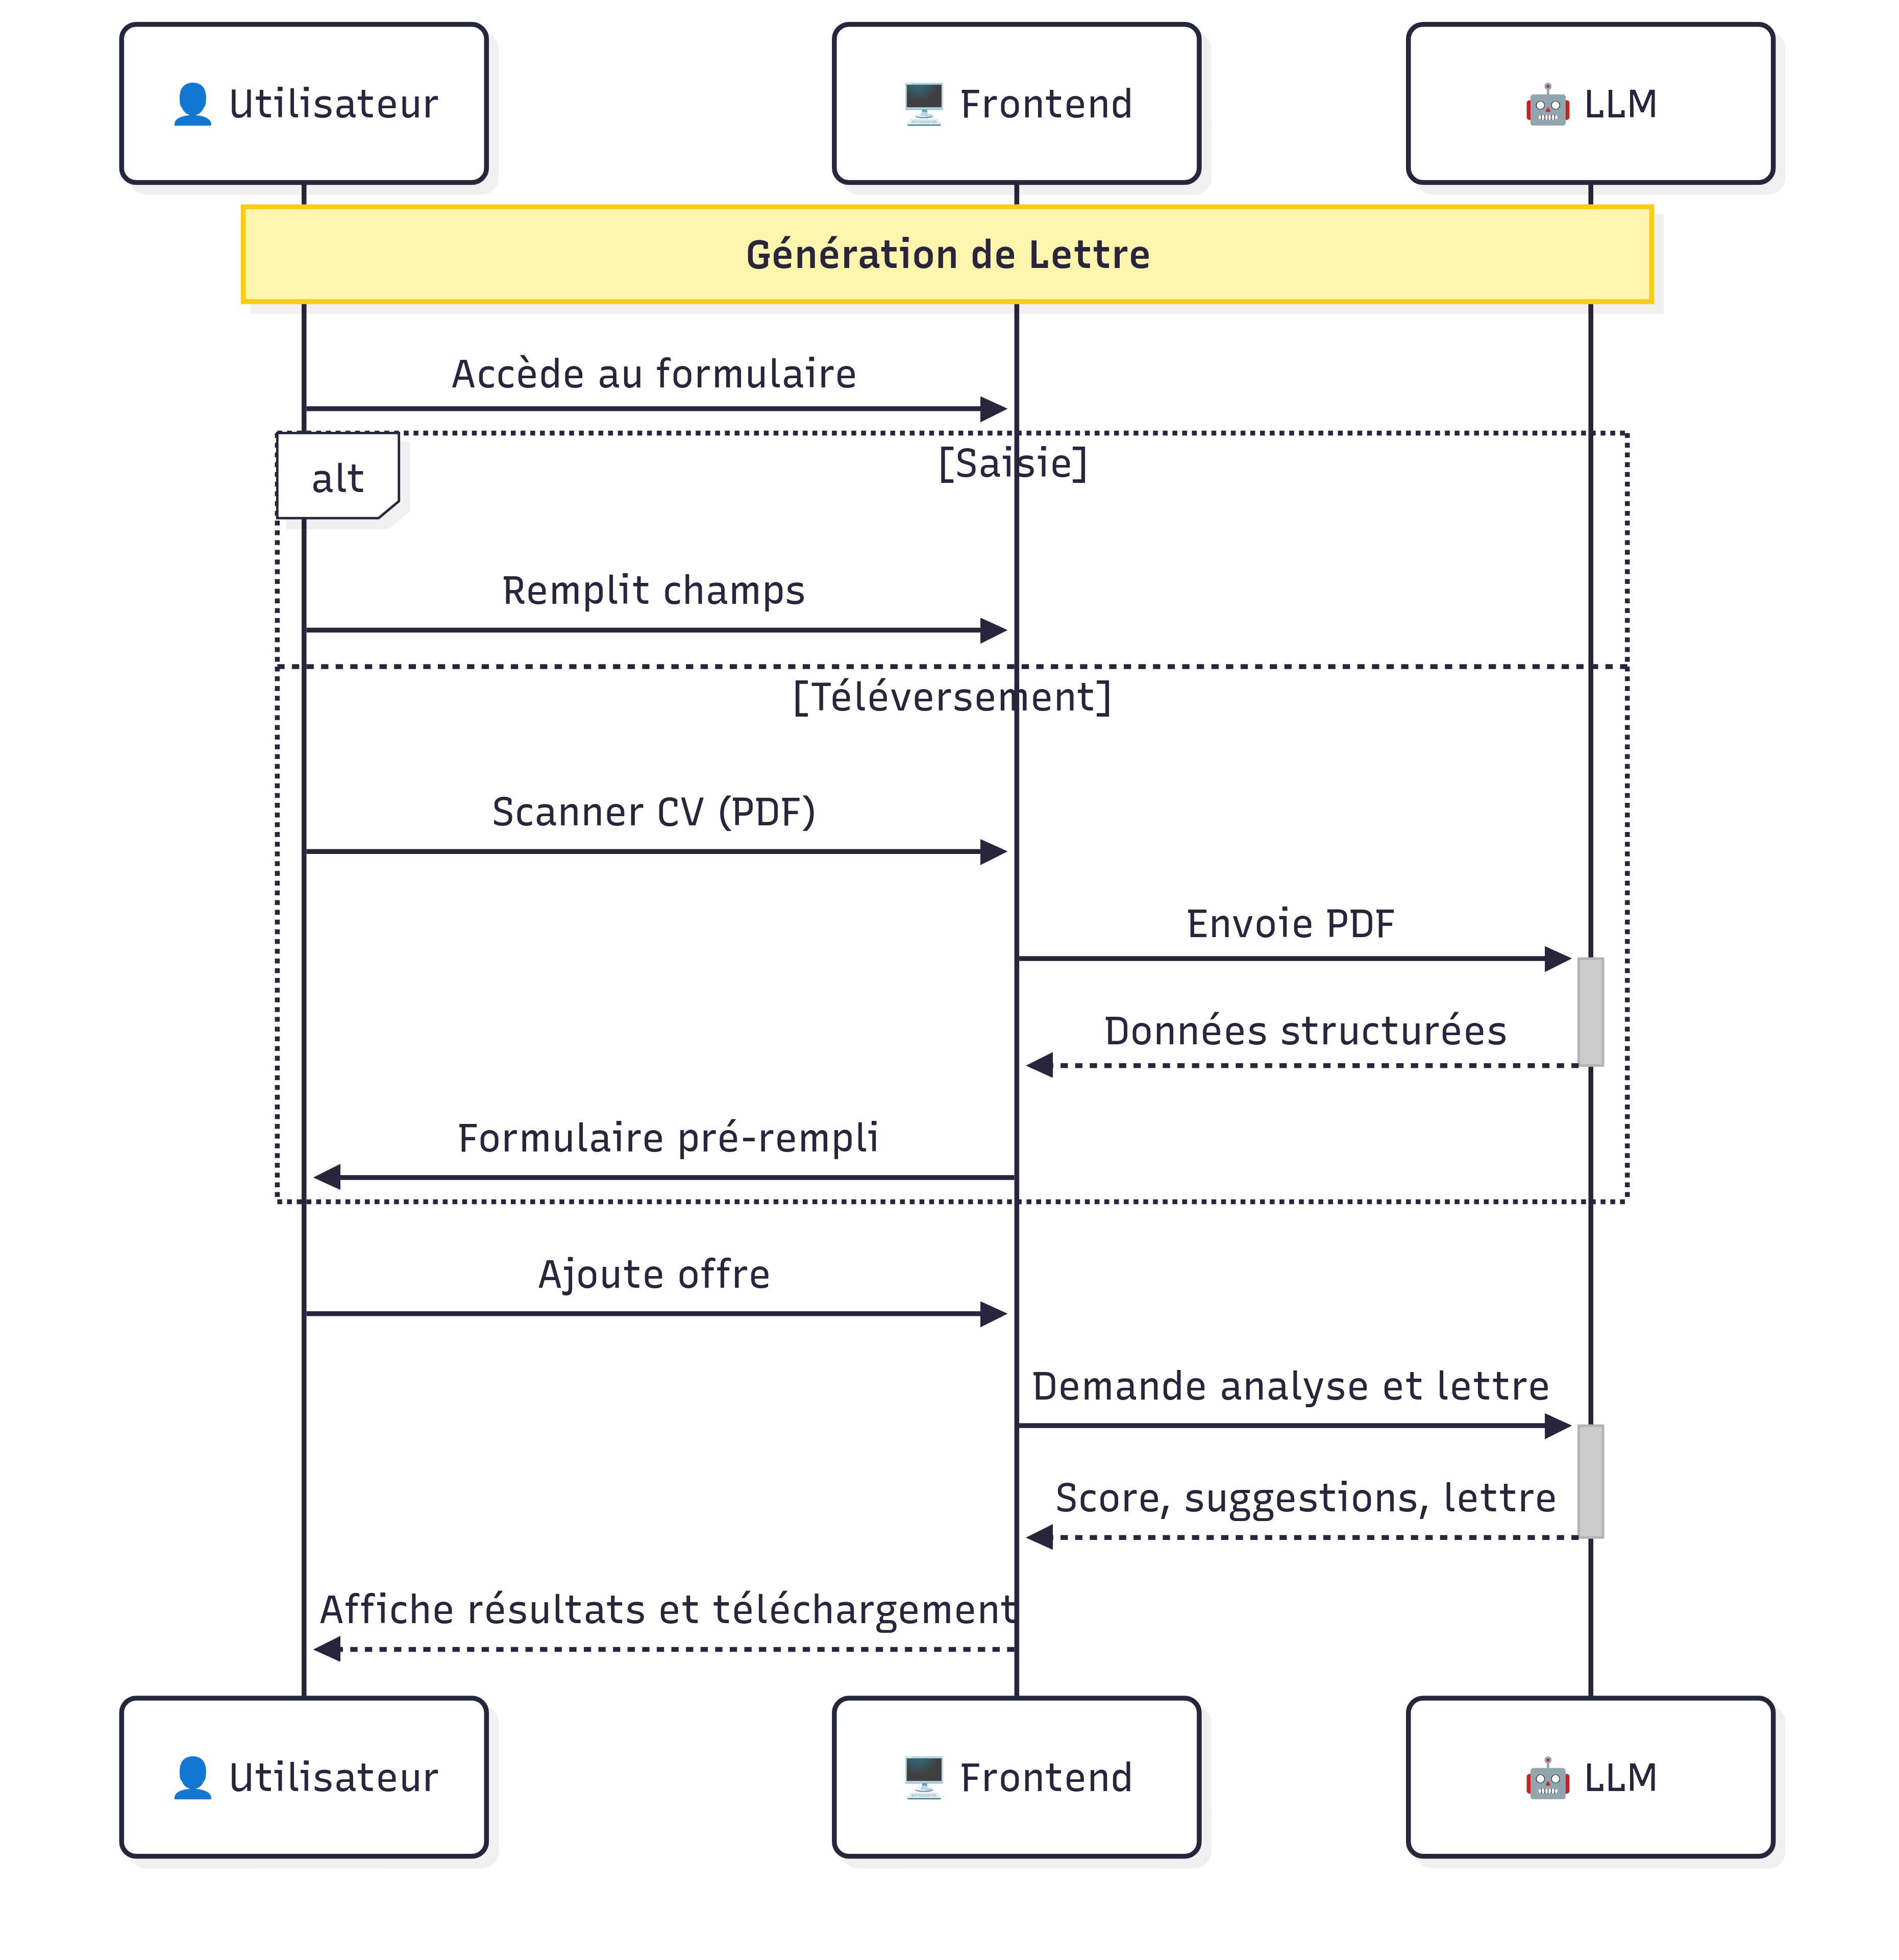
\includegraphics[width=0.8\linewidth]{screens/seqence-Lettre.png}}
    \caption{Architecture de la solution}
    \label{fig:Architecture_de_la_solution}
\end{figure}

\subsubsection*{Acteurs}
\begin{itemize}
    \item \textbf{Utilisateur} : Demandeur d'emploi souhaitant générer une lettre de motivation
    \item \textbf{Frontend} : Interface utilisateur web de la plateforme JobAI
    \item \textbf{Backend} : Service de traitement et orchestration des données
    \item \textbf{LLM} : Modèle de langage Gemini 1.5 Flash pour la génération de contenu
\end{itemize}

\subsubsection*{Prérequis}
\begin{itemize}
    \item L'utilisateur dispose d'un CV enregistré dans la plateforme
    \item Une offre d'emploi cible a été identifiée
    \item L'utilisateur est authentifié sur la plateforme
\end{itemize}

\subsubsection*{Étapes du scénario}

\begin{enumerate}
    \item L'utilisateur accède au module \og Génération de Lettre \fg{} depuis le tableau de bord principal
    
    \item Le système affiche le formulaire de génération avec les options suivantes :
    \begin{itemize}
        \item Saisie manuelle des informations de l'offre
        \item Téléversement d'un CV existant (PDF)
    \end{itemize}
    
    \item L'utilisateur choisit sa méthode préférée et renseigne les champs requis :
    \begin{itemize}
        \item \textbf{Si saisie manuelle} : remplissage du formulaire avec les détails de l'offre
        \item \textbf{Si téléversement} : sélection et upload du fichier CV (PDF)
    \end{itemize}
    
    \item Le Frontend transmet les données saisies au service Backend via une requête API sécurisée
    
    \item \textbf{Si CV téléversé} : Le Backend déclenche le processus de scan et d'extraction :
    \begin{itemize}
        \item Analyse du document PDF
        \item Extraction des données structurées (compétences, expériences, formation)
        \item Structuration des informations au format JSON
    \end{itemize}
    
    \item Le Backend prépare le formulaire pré-rempli en fusionnant :
    \begin{itemize}
        \item Les données extraites du CV
        \item Les informations de l'offre d'emploi
        \item Le profil utilisateur existant
    \end{itemize}
    
    \item L'utilisateur valide et complète les informations affichées dans le formulaire pré-rempli
    
    \item L'utilisateur ajoute les détails spécifiques de l'offre d'emploi cible (entreprise, poste, exigences)
    
    \item Le Frontend envoie l'ensemble des données validées au Backend pour traitement
    
    \item Le Backend formule une requête structurée vers l'API du modèle LLM incluant :
    \begin{itemize}
        \item Le prompt de génération de lettre de motivation
        \item Les données du profil candidat
        \item Les informations de l'offre d'emploi
        \item Les paramètres de personnalisation
    \end{itemize}
    
    \item Le modèle LLM analyse les données et génère :
    \begin{itemize}
        \item Une lettre de motivation personnalisée
        \item Un score de compatibilité profil/offre
        \item Des suggestions d'amélioration du profil
    \end{itemize}
    
    \item Le Backend reçoit la réponse du LLM et effectue les traitements suivants :
    \begin{itemize}
        \item Validation et formatage de la lettre générée
        \item Sauvegarde dans la base de données utilisateur
        \item Préparation des métadonnées (score, suggestions)
    \end{itemize}
    
    \item Le système affiche à l'utilisateur :
    \begin{itemize}
        \item La lettre de motivation générée avec prévisualisation
        \item Le score de compatibilité calculé
        \item Les suggestions d'optimisation personnalisées
        \item Les options de téléchargement (PDF, Word)
    \end{itemize}
    
    \item L'utilisateur peut :
    \begin{itemize}
        \item Télécharger la lettre au format souhaité
        \item Modifier le contenu avant téléchargement
        \item Sauvegarder pour usage ultérieur
        \item Générer une nouvelle version avec des paramètres différents
    \end{itemize}
\end{enumerate}

\subsubsection*{Résultats attendus}
\begin{itemize}
    \item Génération d'une lettre de motivation personnalisée et professionnelle
    \item Évaluation de la compatibilité entre le profil candidat et l'offre
    \item Recommandations pour améliorer l'adéquation du profil
    \item Document prêt à l'emploi disponible en plusieurs formats
\end{itemize}

\subsubsection*{Cas d'exception}
\begin{itemize}
    \item \textbf{Échec de scan PDF} : Message d'erreur et suggestion de saisie manuelle
    \item \textbf{Indisponibilité du LLM} : Notification à l'utilisateur et mise en file d'attente
    \item \textbf{Données insuffisantes} : Demande de complétion du profil utilisateur
\end{itemize}

% \begin{figure}
% 	\centering
% 	\begin{subfigure}[b]{0.45\textwidth}
% 		% \includegraphics[width=\textwidth]{screens/login.png}
% 		\caption{Page de connexion}
% 		\label{fig:login}
% 	\end{subfigure}
% 	\hfill
% 	\begin{subfigure}[b]{0.40\textwidth}
% 		% \fbox{\includegraphics[width=\textwidth]{screens/signup.png}}
% 		\caption{Page d'inscription}
% 		\label{fig:signup}
% 	\end{subfigure}
% 	\caption{Authentification utilisateur}
% 	\label{fig:auth}
% \end{figure}

